\documentclass{report}

\usepackage[utf8]{inputenc}
\usepackage[T1]{fontenc}
\usepackage[francais]{babel}
\usepackage{graphicx}
\usepackage{lmodern}
\usepackage{amsmath}
\usepackage{amssymb}
\usepackage{mathrsfs}
\usepackage{geometry}
\geometry{scale=0.8, nohead}

\author{Gautier \bsc{Dakin}, Nicolas \bsc{Ehrhardt}}
\title{Projet Gherkin}

\begin{document}
\maketitle

\tableofcontents


\chapter{L'interface graphique}
\section{Orientation du projet}
Comme sus-mentionné nous avons basé notre interface sur celle du lecteur audio par défaut (type Rhythmbox, de sorte à ne pas perturber les habitudes de l'utilisateur). Mais un constat s'impose : Aujourd'hui, les écran 16/10 voire 16/9 sont légions et majoritaires ; Ubuntu, à travers unity, à décidé de tirer parti de ce nouvel état de fait pour proposer un menu latéral. Les arguments sont : gain de place, minimalisme. Le principal problème étant que ce menu empiète parfois sur les boutons des applications en plein écran lorsque celui-ci se dévoile.

Pour répondre à cette problèmatique, nous proposons un menu à droite de notre application. Optimisant ainsi la place, et évitant cette gène.

\section{Développement}
La librairie PyQt4 sur laquelle se base le lecteur nous a permis de développer rapidemment cette interface. Le développement de l'interface s'est fait en trois temps :
\begin{enumerate}
\item On crée dans un premier temps une première interface graphique grâce à QtDesigner. Cette application permet d'avoir une vision en WYSIWYG (\emph{What you see is what you get}) de l'interface, et donc d'éviter les erreurs de goûts et de mauvais placement.
\item On modifie légèrement le code généré par QtDesigner pour rajouter quelques fonctionnalités. (Ex : Gestion des îcones)
\item On sépare le fichier en deux .py. Un premier contient le code légèrement modifié obtenu via QtDesigner. Le second va gérer toutes les modifications de l'interface graphique, ainsi que la gestion des signaux et slots de Qt. (Ex : l'update de la barre de progression, lié le PlayButton à la fonction play(),... )
\end{enumerate}

\begin{figure}[h]
\centering
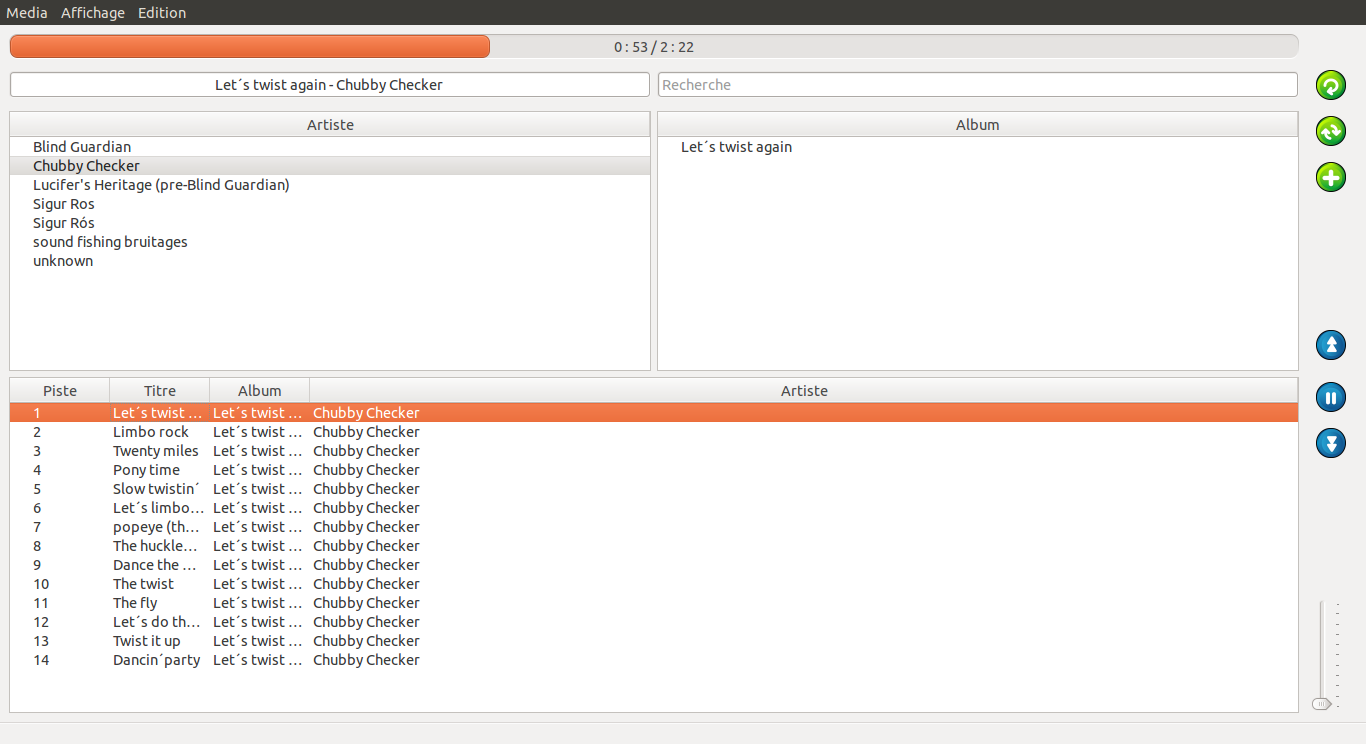
\includegraphics[scale=.3]{interface.png}
\caption{Interface graphique du lecteur.}
\end{figure}


Nous avons, en outre, rajouté plusieurs fenêtres supplémentaires. Une première fenêtre permet de pouvoir sélectionner l'endroit où se trouve la musique (DDE, Dossier Musique, ...) afin que l'utilisateur puisse mettre à jour sa base de données sans avoir à passer par le mode console. Une seconde fenêtre a été créée et permet à l'utilisateur de pouvoir voir l'état de la playlist en cours de lecture, de la modifier si besoin en ôtant ou en rajoutant des éléments. Enfin une dernière fenêtre permet de rentrer l'adresse IPv4 d'un serveur pour pouvoir directement écouter la musique depuis le serveur, à condition, évidemment, que l'adresse IP rentrée soit valide.

\chapter{L'intelligence}
\section{L'idée du côté utilisateur}

L'idée de l'intelligence est simple en elle-même. Elle a pour but de mettre des probabilités sur le passage entre deux chansons. Exemple : Vous êtes actuellement entrain d'écouter la "Sonate au Clair de Lune". Théoriquement, la probabilité d'avoir envie d'entendre/écouter "Highway to Hell" après la "Sonate au Clair de Lune" est extrêmement faible (sauf si cela est dans vos habitudes).
Si, au contraire, après la sonate de Beethoven, l'utilisateur a tendance à écouter le "Requiem" de Mozart, alors la probabilité de passage entre ces deux chansons sera d'autant plus grande.

Cette vision de passage d'une chanson à l'autre entre exactement dans le cadre théorique des chaînes de Markov où l'on a une matrice P tel que $P(x,y)$ représente la probabilité de passage de l'état x à l'état y.

\subsection{Développement}

On a donc l'idée de représenter les transitions entre deux pistes audio par une chaine de Markov. Reste à savoir comment l'implémenter. Imaginons une bibliothèque moyenne sur un ordinateur. On tourne autour de $4000 -- 5000$ pistes audio. Gérer en permanence une telle matrice est extrêmement lourd, or on recherche en premier la rapidité d'exécution. On développe donc comme suit :

\begin{itemize}
\item
On crée un dictionnaire de nom markov, tel que $markov[i][j]$ renvoie la probabilité de passage de $i$ à $j$ si elle existe.
\item
On pondère ces probabilités par un nombre dépendant uniquement de i. Ce choix implique qu'on considère qu'à un temps très élevé, on a théoriquement convergence vers la playlist idéale pour l'utilisateur. Cela ne signifie pas pour autant que la playlist devient déterministe. On a juste théoriquement élagué les probabilités très faibles pour ne laisser plus que les probabilités plus importantes. On a donc en théorie une convergence vers un arbre de probabilité plus ou
moins stable par utilisation de Gherkin.
\item
Selon certains critères, on décide d'incrémenter ou de décrémenter la probabilité, en gardant le caractère stochastique de markov. On incrémente ainsi la probabilité lorsque l'on réalise l'écoute entière d'un morceau, on incrémente la probabilité entre le morceau précédent et ce morceau. Lorsque l'utilisateur décide de passer une chanson, on abaisse la probabilité de passage entre le morceau précédent et le morceau qui vient d'être sauté. Enfin, on décide
d'incrémenter la probabilité lorsqu'un morceau est double cliqué, ce qui peut permettre à l'utilisateur de configurer en quelques instants ces playlists.
\item
Régulièrement, on enregistre le dictionnaire markov sur le disque dur. Enfin d'éviter de revenir au cas de la matrice, les probabilités trop faibles ($ < \epsilon$) sont élaguées c'est-à-dire qu'elles sont suppriméees et rajoutées équiprobablement sur les autres clefs du dictionnaire. Cet élagage permet de réduire le nombre de clefs du dictionnaire et donc de garantir une taille plus faible.
\end{itemize}


\section{L'idée du côté serveur}

Du côté utilisateur, on ne se focalise que ses préférences personnelles. Du côté serveur, on ne peut se permettre de faire cela. Certes, on pourrait considérer la moyenne des préférences des utilisateurs, mais ce ne serait qu'un vulgaire plagiat de ce qu'un grand nombre de lecteurs audio sur Internet fait.

Nous avons donc fait le choix de faire du machine-learning sur les bases de données, c'est-à-dire essayer par un algorithme de machine-learning de classifier les chansons, et des les isoler en sous-groupes pertinents afin de faciliter le stockage et permettre à l'utilisateur une utilisation intéressante.

Pour se faire, nous avons besoin de pouvoir créer des données à classifier par un quelconque algorithme. On utilise pour faire cela la bibliothèque Yaafe. Cette bibliothèque permet d'extraire 22 constantes propres à chaque chanson qui détermine son rythme, son timbre et ses sonorités. On obtient donc après traitement des données, une immense matrice de 22 colonnes et d'autant de lignes que de chansons dans la base de données.

Il faut désormais traiter cette matrice. Les algorithmes qui nous apparaissent comme pertinents dans le cadre d'une classification d'oeuvres musicales sont les algorithmes de clustering.

Le clustering consiste à créer des sous-groupes de données au sein d'un immense jeu de données, et donc d'attribuer ici à chaque morceau de musique, un cluster ou un groupe d'appartenance. L'intérêt du clustering est qu'il nous permet donc de dire qu'un morceau appartient à tel sous groupe et donc qu'à la fin de la lecture de ce morceau, la probabilité est assez forte de rester au sein de ce groupe, puisqu'ils sont en théorie assez proche musicalement parlant, il existe ensuite une probabilité, plus faible, de quitter ce cluster et d'aller en rejoindre un autre. Plus ce second cluster sera proche du premier en terme de distance "musicale" toujours, plus la probabilité sera proche.


Les algorithmes retenus sont issus d'une bibliothèque du logiciel $R$ (la librairie cluster). Ils sont au nombre de 3 : k-means, pam et fanny.

\subsection{K-means}

L'algorithme K-means consiste à dire qu'un morceau de musique appartient à un groupe noté $\mathfrak{G}$ si et seulement si la majorité de ses k-plus proches voisins sont aussi dans le groupe $G$. C'est donc un algorithme basique (presque naïf) qui a l'immense avantage d'être rapide comparé aux deux autres algorithmes, bien que l'algorithme sont moins stables que les deux autres.

Concrètement en projetant le résultat obtenu dans les deux premières dimensions, on obtient un graphique de ce type. Chaque rond y représente un morceau de musique, chaque étoile un cluster qui donne sa couleur à son groupe.

ATTENTION PENSER A INSERER L'IMAGE PROPREMENT DITE

\subsection{Fanny (Fuzzy Analysis clustering)}

L'algorithme Fanny ne classifie pas directement un morceau comme appartenant à un groupe $G$ mais en donnant à la place la probabilité pour un morceau d'appartenir à tel ou tel groupe (ou cluster). On peut ensuite apprendre le cluster en prenant le cluster qui maximise cette probabilité. L'avantage de ces probabilités est qu'elles permettent de voir la pertinence de l'appartenance d'un morceau à tel ou tel cluster, et semble être un peu moins sélectif que le cas normal.

\subsection{Pam}

Bla bla sur les médoides


\subsection{Chaîne de Markov}

En sortie de ce clustering, on souhait obtenir une nouvelle chaîne de Markov, telle que $markovS[i][j]$ représente la probabilité de passage du morceau $i$ au groupe de musique $j$. Il suffira ensuite de sélectionner une musique aléatoirement ou selon les préférences de l'utilisateur dans ce groupe de musique et de la jouer. Dans le cas où l'on utiliserait en sortie le custering de fanny, on aurait directement cette chaîne de Markov. Sinon, pour les deux autres algorithmes, il suffirait de la construire, en se basant sur la distance entre les clusters (qu'elle soit calculée entre les deux plus proches éléments, les deux plus éloignés ou en moyenne).


\chapter{Architecture en client/serveur}


\chapter{Langages et bibliothèques utilisés}

\section{Langages de programmation}
\subsection{Python}

\subsection{Bash}

\subsection{XML}

\subsection{R}

\section{Bibliothèques}

\subsection{GStreamer}

\subsection{Yaafe}

\subsection{XMLRPC}

\subsection{ConfigParser}

\subsection{Cluster (R)}

\chapter{Historique de Gherkin}


\chapter{Les grandes lignes du code}
% DOXYGENE

\end{document}
